% !TEX root =  main.tex

%Description of \m\mEdhoc and main changes from last verified version

\vnote{Note for discussion with others: I find the macros for the protocol, method, and tool names distracting while reading through (the font changes too much, too often). The macro for EDHOC actually inserts a line break if you start a sentence with it, because of the \texttt{hbox} (I'm not sure why the hbox exists for what is a macro to be inserted in running text). I do need to start sentence with EDHOC many times though, so this is irritating. It is also the case that ProVerif needs to be written like so, and not capitalized entirely, so at least one of them is plain wrong! For now I've left in the macros, but I'd prefer that we fixed them to be regular capitalized text or, in the case of ProVerif, in camelcase as they should be.}

\vnote{Macros don't work right in section headers!}

\subsection{Overview}
Constrained IoT systems often deal with a lot of valuable personal and business information that ought to be kept secure. Such systems need to be assured of end-to-end protection with source authentication and perfect forward secrecy. It is often desirable to protect such devices at the application layer -- for example, in cases where transport layer security is not sufficient, or where multiple underlying protocols need to be accounted for. One method for providing application layer security is provided by CBOR Object Signing and Encryption (\mCose)~\cite{rfc8152}.  

In order to derive shared key material with which to proceed, communicating parties can run an Elliptic Curve Diffie-Hellman key exchange protocol with ephemeral keys. Ephemeral Diffie-Hellman Over \mCose (\mEdhoc) is a lightweight key exchange protocol for such situations, and is expected to provide perfect forward secrecy and identity protection. \mEdhoc supports authentication using pre-shared keys (PSK), raw public keys (RPK), and public key certificates. After successful completion of the \mEdhoc protocol, application keys and other application specific data can be derived using the \mEdhoc-Exporter interface. 

A main use case for \mEdhoc is to establish a security context for Object Security for Constrained RESTful Environments (\mOscore)~\cite{rfc8613}. \mOscore is a protocol which uses \mCose for application-layer protection on top of the transport-layer Constrained Application Protocol (CoAP). \mEdhoc uses \mCose for cryptography, CBOR for encoding, and CoAP for transport. By reusing existing libraries, the additional code footprint can be kept very low.

\mEdhoc is designed to work in highly constrained scenarios. This makes it especially suitable for network technologies which have low throughput, low power consumption, and small frame sizes. Examples include Cellular IoT, 6TiSCH, and LoRaWAN~\cite{lorawan1,lorawan2}.

The \mEdhoc protocol can establish Diffie-Hellman key exchange in one of three different ways -- using digital signatures, static Diffie-Hellman (DH) keys, or pre-shared symmetric keys. We describe each of these methods in detail below. The communicating parties must agree on the method and cipher suite used for encryption as part of the first message. The parties exchange ephemeral public keys, compute the shared secret, and derive symmetric application keys from this secret.

The \mSigma (SIGn-and-MAc) family of protocols~\cite{sigma} has many variants. The \mSig-based methods of \mEdhoc are built on \mSigmaI, a variant of the \mSigma protocol which provides identity protection for the initiator, and  implements the \mSigmaI variant as Mac-then-Sign. The method involving static DH keys proceeds along the lines of \mOptls, with the agent creating a MAC and encrypting it using an algorithm for authenticated encryption with associated data (\mAead)~\cite{aead,rfc5116}. 

\mEdhoc allows the initiator and responder to run different methods, combining \mSig and \mStat -- for example, the initiator might run a \mSig-based method, while the responder is running a \mStat-based method. This set of methods is not covered in previous versions of \mEdhoc, which only had a single \mSigma asymmetric key method (corresponding to the \mSigSig method shown in Section~\ref{sec:methods}). This allows one party to use a \mSigma style of authentication using signatures, while the other can use static DH keys. In Figure~\ref{fig:edhocasym}, a template for all the asymmetric key methods of EDHOC is shown. 

\begin{figure}[!h]\label{fig:edhocasym}
\centering
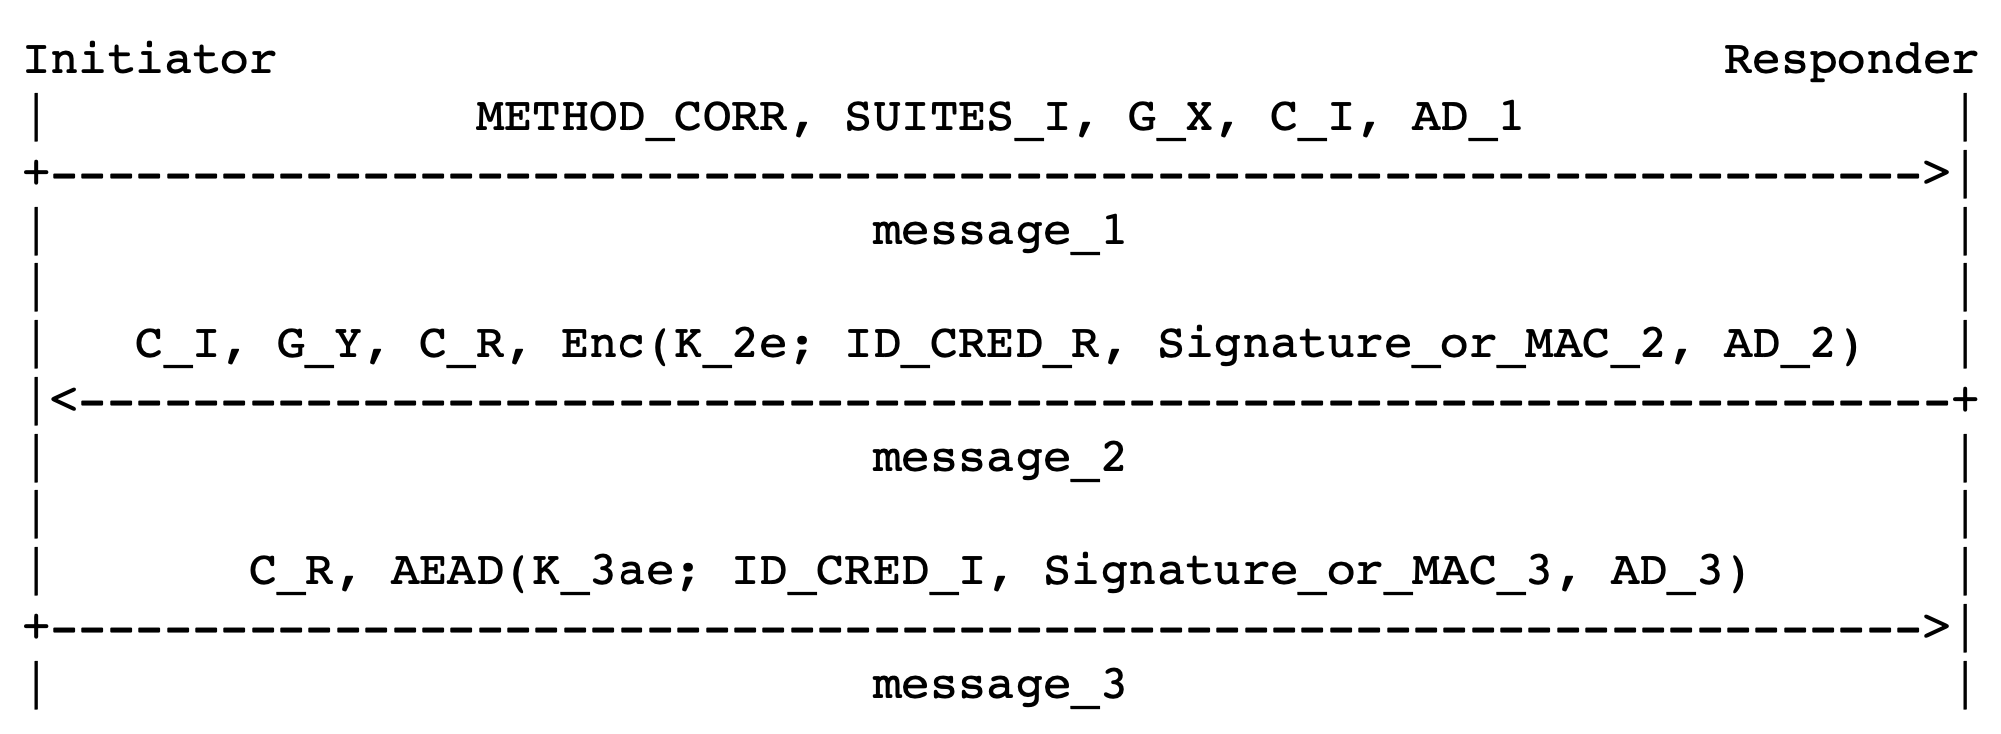
\includegraphics[scale=0.3]{Images/asym.png}
\caption{A template for the asymmetric key methods of EDHOC}
\end{figure}

\subsection{Background, comparison with~\cite{DBLP:conf/secsr/BruniJPS18}}
The first version of \mEdhoc was proposed in March 2016 to a working group investigating lightweight authenticated key exchange protocols [\mcneed]. There has been a focus on formally verifying that the protocol satisfies the properties expected of it right from the beginning. 

The 2018 work~\cite{DBLP:conf/secsr/BruniJPS18} by Bruni et al performed a formal verification of version 08 (\url{https://tools.ietf.org/html/draft-selander-ace-cose-ecdhe-08} \mcfix) of \mEdhoc. The protocol and properties are modelled and verified in the \mProverif tool. This version of the protocol belongs to the \mSigmaI family of protocols, and has two modes -- one with asymmetric keys, and one with pre-shared symmetric keys. Bruni et al showed that this version satisfies the requisite properties of identity protection, (perfect forward) secrecy of data, and strong authentication, upon completion of the protocol.

\mEdhoc has undergone a lot of change since version 08, as will be described in the following sections, and the formal verification of the current version, therefore, is a worthwhile exercise.

\subsection{Comparison with \mOptls and \mNoise}
\vnote{Would this perhaps be better served by putting it in related work?}
\knote{To me, related work is about work related to \emph{our} work, i.e., that
    section is about relations between our analysis of \mEdhoc{} and other
    \emph{analysis} of protocols (analysis of \mEdhoc{} in particular).
    Relations between \mEdhoc{} itself as a protocol and other protocols is
    part of the object/subject we are studying. It is part of our analysis to
    study those relations. So I think it belongs here.}

\section{Methods and features of \mEdhoc}\label{sec:methods}

\subsection{Fundamental components of \mEdhoc}
\subsubsection{\mCose}
\mCbor is a data format designed for small code size and small message size. The \mCbor Object Signing and Encryption (\mCose) protocol is used to create and process signatures, MACs, and encryption using CBOR. 

A \mCose object contains bitstrings corresponding to protected parameters (which ought to be cryptographically protected), unprotected parameter, and the payload to be signed. This can be signed/encrypted/MACed, to obtain a resultant \mCose object containing the bitstring corresponding to the operation. The respective algorithms may also be fed some externally supplied data, which is carried along with the \mCose object, but is not part of it. \mEdhoc only uses the signature and encryption objects of \mCose. For encryptions, \mCose supports two different methods -- one where the recipient is not needed because the key is known implicitly, and one for all other cases. \mEdhoc only uses the former. 

A \mCoseEncrypt structure as used in \mEdhoc is a \mCbor array with a text field which contains the string ``Encrypt0'' to denote the use of the method with implicit recipient, a field for protected data, a field for externally supplied application data, and a field for ciphertext. All these fields store the corresponding bitstrings.

\subsubsection{\mAead}
Authenticated encryption with associated data, or \mAead, is an authenticated encryption operation. The algorithm takes in a key, a unique nonce, a plaintext, and some associated data, and outputs a ciphertext. The plaintext is both authenticated and encrypted, while the associated data is merely authenticated. The ciphertext is at least as long as the plaintext. When the plaintext is empty, the \mAead algorithm acts as a MAC on the associated data. 

The associated data is used to protect information that needs to be authenticated, but does not need to be kept confidential. It might be desirable to authenticate this information, although it must be left unencrypted to allow the system to function properly. Authentication is provided without copying the data into the plaintext.

\subsubsection{Key derivation function (KDF)}
Perhaps the most important building block for \mEdhoc is the key derivation function based on \mHkdf~\cite{rfc5869}, which is used to generate the pseudorandom strings and keys for the encryption operations in the communicated messages. The pseudorandom strings (\mPRKtwo and \mPRKthree) are derived using the \mHkdf-Extract function, while the keys are generated using the \mHkdf-Expand function. Both these functions are based on \mHmac~\cite{rfc2104}, which is a hashing system for message authentication.

The \mHkdf-Extract function is run with a salt and some input keying material (IKM) as input. It produces as output a pseudorandom string. For the \mPskPsk method alone, the salt is the key pre-shared between the initiator and the responder, while for the other methods, it is empty. The IKM for all \mEdhoc methods is the ECDH shared secret \mGxy.

In order to generate keys for the various encryptions, the \mHkdf-Expand function is used. This is run with a pseudorandom string, an info string, and the length of the output keying material (OKM) as input. The pseudorandom string is generated using \mHkdf-Extract as above. The info string contains details of the \mAead encryption algorithm used, length of the OKM, and the transaction hash as used for the specific method (a detailed discussion follows, for each method). In case the length $l$ of the OKM is shorter than that of the transaction hash, the OKM is obtained by taking the first $l$ bits of the result of running \mHmac on the pseudorandom string, and a concatenation of 0x01 and the info strings.

We now discuss each of the \mEdhoc methods in detail over the next few sections.

\subsection{\mPskPsk method}
In this method, the initiator and responder are assumed to have a pre-shared key (PSK) which is secret to them, and can be retrieved by the responder using a public part of the first message (\mIDPSK). This method corresponds to the symmetric key method of \mEdhoc v08. 

In the first message, the initiator sends a message consisting of the method name, the cipher suites ranked in order of preference, the initiator's ephemeral key (\mGx), their connection identifier (\mCi), the \mIDPSK identifier, and (optional) auxiliary data (\mADone). The responder, upon receipt of this message, must verify that the selected cipher suite is supported,  and pass \mADone to the security application which needs it. If any verification step fails, the initiator sends an EDHOC error message back, and the protocol aborts.

The second message, sent by the responder, is composed of \mCi, the responder's ephemeral key \mGy, their connection identifier \mCr, and a \mCose object. This contains as external data the transaction hash of the first message (\mTHtwo), along with an \mAead encryption of the (optional) auxiliary data \mADtwo. The key used for this (\mKtwo) is derived using the EDHOC key derivation function with \mTHtwo and the pseudorandom string \mPRKtwo as input, while the associated data for the \mAead encryption is constructed by concatenating a constant string, plaintext \mhplain, and \mTHtwo. Recall that the PRKs in this method are constructed by running \mHkdf-Extract using PSK as salt. 

The initiator, upon receipt of this message, sends back \mCr, followed by a \mCose object containing an \mAead encryption of auxiliary data \mADthree, along with the transaction hash of the second message (\mTHthree) as external data. As earlier, the key used is derived by supplying \mTHthree and \mPRKthree as input to the KDF, and the associated data obtained by concatenating the constant string, plaintext \mhplain, and \mTHthree. An abstract description is shown in Figure~\ref{fig:edhocpsk}.

\vnote{Figure numbers don't square up, check class file guidelines!}

\begin{figure}[!h]\label{fig:edhocpsk}
\centering
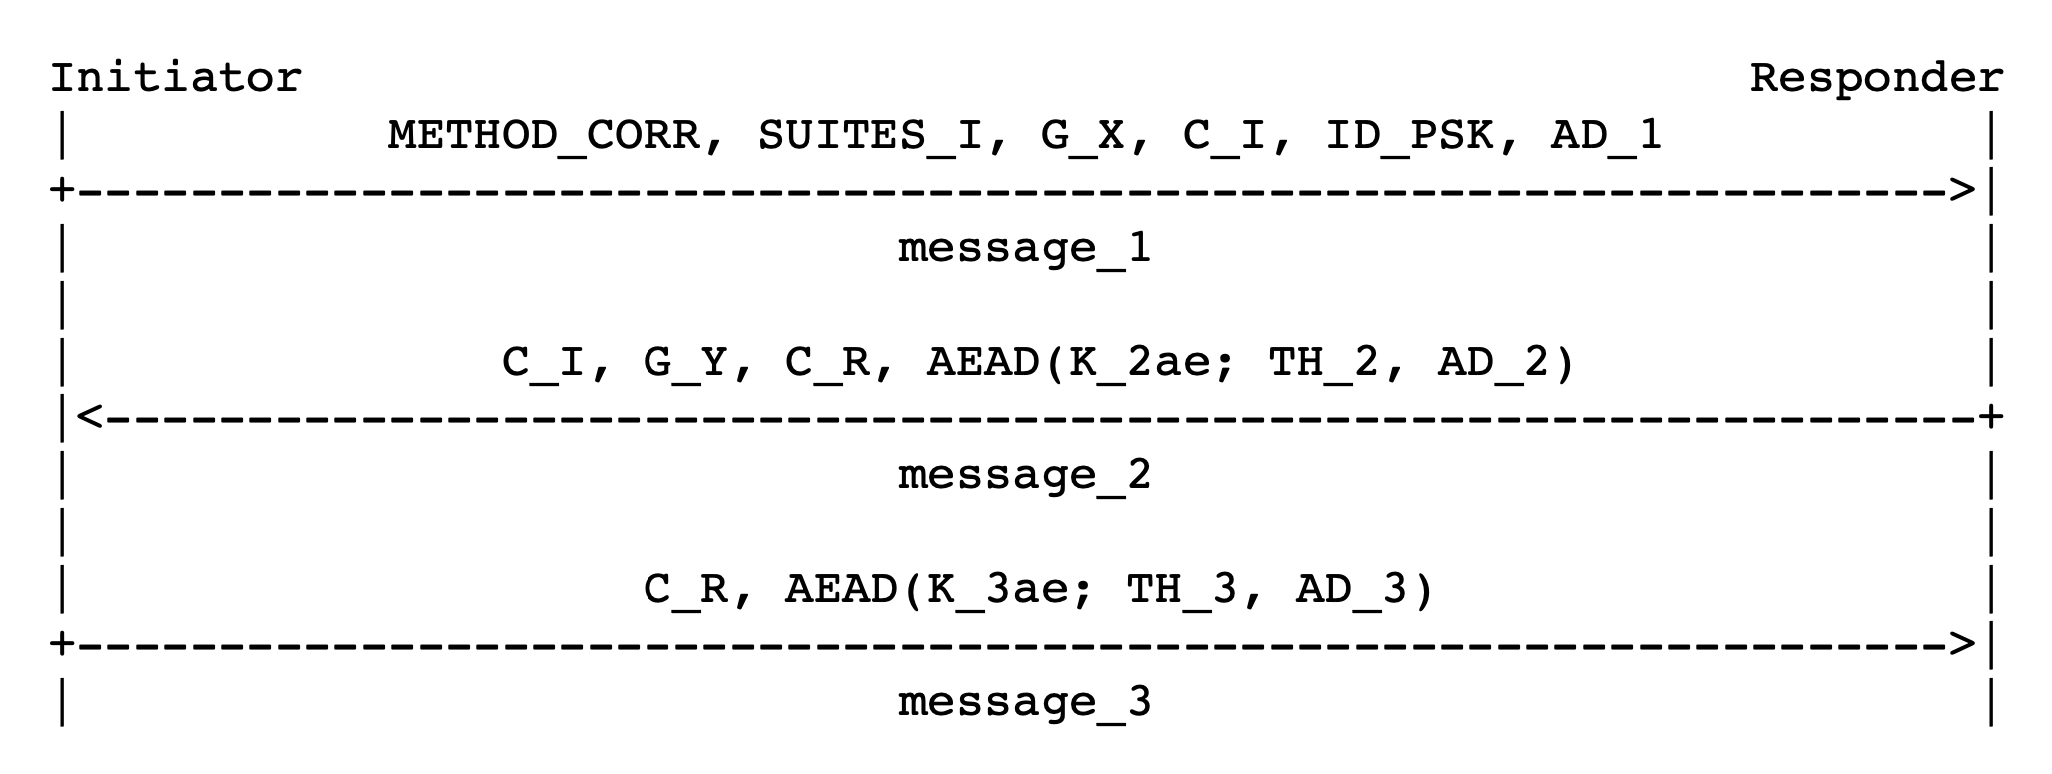
\includegraphics[scale=0.3]{Images/psk.png}
\caption{The PSK-PSK method of EDHOC}
\end{figure}

\subsection{\mStat-based methods}
\mEdhoc allows for three \mStat-based methods -- two where only one participant has a static Diffie-Hellman key (while the other uses signatures), and one where both do. 

In the first message, the initiator includes an identifier for the method, a preference-ordered list of cipher suites, their ephemeral key \mGx, their connection identifier \mCi, and some optional plaintext \mADone. This message is common to all the four methods below involving asymmetric keys. 

The responder, upon receipt, verifies the cipher suites, passes any \mADone to the application that needs it, and proceeds to construct and send the second message. This message contains (not necessarily all of) \mCi, \mGy, \mCr, and an encrypted term. The initiator, upon getting this message, sends out a message containing an encrypted term. Depending on the methods being run by the initiator and responder, the exact contents of these messages may vary. We will now describe each of these methods and the second and third messages therein in detail.

\subsubsection{\mSigStat}
The initiator runs a \mSigma-based method, with signatures, while the responder operates with a static Diffie-Hellman key and MACs. Since this method is one where the responder runs \mStat, in the second message, \mCi is omitted. The encrypted term for the second message is constructed as follows. 

First, we build the \mCose object that is the inner MAC, since the responder runs \mStat. The protected part of this object is an identifier for retrieving the responder's public authentication key \mCredr. The externally supplied data is the transaction hash \mTHtwo of the first message and \mGy,  the responder's public authentication key \mCredr, and (optional) auxiliary data \mADtwo. The key used for the encryption is the output of the KDF on being fed as input the pseudorandom string \mPRKthree and \mTHtwo. The resulting encrypted object is now referred to as the ciphertext \mMactwo. 

For the outer encryption object, we consider the plaintext formed by concatenating the bitstrings corresponding to the identifier for \mCredr, \mMactwo, and \mADtwo (if any). The encryption is obtained by performing an \mXor operation on this plaintext with the key \mKtwo, which is obtained by using the KDF on \mPRKtwo and the transaction hash \mTHtwo. The responder therefore sends to the initiator \mGy, \mCr, and this \mCose encryption object as the second message.

The initiator responds with the third message, consisting of \mCr, and an encrypted object. Here, again, we first build the inner \mCose object. This process is analogous to that employed by the responder for the second message. The \mCose object has as protected data an identifier for retrieving the initiator's public authentication key \mCredi. The externally supplied data is the transaction hash \mTHthree of the second message and \mTHtwo,  the initator's public authentication key \mCredi, and (optional) auxiliary data \mADthree. The key used is obtained by inputing the pseudorandom string \mPRKfour and \mTHthree. The resulting encrypted object is now referred to as the ciphertext \mMacthree. 

Since the initiator is running \mSig, this \mCose object needs to be signed. To the signing algorithm, the initiator sends as protected data the identifier for retrieving \mCredi, as external data the concatenation of \mTHthree, \mCredi, and any \mADthree, and the payload \mMacthree. This is signed using the private authentication key of the Initiator.  

We now construct the encryption for the third message, by passing to an \mAead encryption algorithm a \mCose object with no protected data, external data \mTHthree, and a plaintext obtained by concatenating the identifier for retrieving \mCredi, the signed object described above, and \mADthree. The key used for encryption is \mKthree, obtained by running the KDF on the pseudorandom string \mPRKthree and \mTHthree. Thus, the message sent by the initiator to the responder in the third step is \mCr accompanied by this encrypted object.

\subsubsection{\mStatStat}
In this method, both the initiator and the responder run the \mStat method. The responder's message looks exactly the same as in the previous subsection, for \mSigStat. The initiator's message, however, is not signed anymore, since the initiator too is running the \mStat method. Thus, we skip the signature process in the steps described above, and instead of passing a signed object to the \mAead encryption algorithm, we pass \mMacthree itself. Everything else stays the same as earlier.

\subsubsection{\mStatSig}
Here, the responder runs the \mSig method, while the initiator runs the \mStat method. Thus, the second message, sent by the responder to the initiator needs an extra layer of signing. Once \mMactwo has been constructed, as in the methods where the responder runs \mStat, the responder runs the signature algorithm with a \mCose object. This object has the identifier for \mCredr as protected data, a concatenation of \mTHtwo, \mCredr, and \mADtwo as external data, and the payload \mMactwo. This is signed using the responder's private authentication key.

The outer encryption object is constructed by considering a plaintext consisting of \mCredr, this signed object (instead of \mMactwo, as was the case when the responder ran the \mStat method), and \mADtwo. \mKtwo is generated the same way as earlier, and the responder sends \mGy, \mCr, and this encrypted object to the initiator as the second message.

Since the initiator is running the \mStat method, there is no change in the third message from the previous case. There is no signature, and only \mMacthree is encrypted via \mAead.

\subsection{\mSigSig method}
In this method, both parties run the \mSig method, and therefore, both the second and third messages need to be signed before being encrypted via \mAead. The second message looks like the one from the \mSigStat method described above, while the third looks like the one from the \mStatSig method.


\vnote{Need to insert tikZ figures}

\subsection{Deriving an OSCORE context}
\mEdhoc is often used to set up parameters for \mOscore. In this case, the parties make sure that the connection identifiers are distinct, i.e. $\mCredi \neq \mCredr$, since these are used as \mOscore sender IDs. If the initiator plays the role of the CoAP client, and the responder the role of the CoAP server, the client gets the sender ID \mCredr and the server the ID \mCredi (the identifiers are swapped). The \mAead and hash algorithms for \mOscore stay the same as those used for the selected cipher suite in \mEdhoc, while the master secret for \mOscore is derived using the key length of the \mAead algorithm of \mEdhoc. 

\subsection{Expected security properties}
\mEdhoc inherits some security properties from the \mSigmaI protocol. These are perfect forward secrecy, mutual authentication with aliveness, consistency, peer awareness (to the responder, but not to the initiator), identity protection, and Key Compromise Impersonation (KCI) resistance.

All methods other than \mPskPsk offer identity protection of the initiator against active attacks and that of the responder against passive attacks. The roles should be assigned to protect the more sensitive identity. This is usually the entity whose identity cannot be inferred from information in the lower layers.

\mEdhoc also provides protection against replay attacks by the attacker. The attacker also cannot affect any negotiated parameters. A single session of \mEdhoc enables the responder to verify that the selected cipher suite is the most preferred of the initiator which is supported by both parties, even though there is no negotiation of cipher suites per se.

In order to reduce the chances of pervasive monitoring, \mEdhoc only supports methods with perfect forward secrecy. One way to limit the effect of breaches is to minimize the use of symmetrical group keys for bootstrapping. \mEdhoc, therefore, uses raw public keys and self-signed certificates instead of symmetrical group keys for bootstrapping.

For the \mPskPsk method, compromising PSK lets the attacker impersonate either party in \mEdhoc exchanges with the other. For the other methods, compromising the private authentication keys of one party lets the attacker impersonate only the compromised party in exchanges with other parties. In particular, it does not let the attacker masquerade as any other parties in communications with the compromised party. 

Compromise of the \mHkdf input parameters (ECDH shared secret and/or PSK) leads to all session keys derived from that shared secret being deemed compromised. However, the compromise of one session key does not affect other session keys. If the long-term keys (PSK or private authentication keys) are compromised, this does not affect the security of instances of \mEdhoc which have completed prior to compromise. 

